% Modified by Alessio Guglielmi, 3 February 2021

\documentclass[12pt,a4paper]{report}
% This document template assumes you will use pdflatex.  If you are using
% latex and dvipdfmx to translate to pdf, insert dvipdfmx into the options.

\usepackage{Bath-CS-Dissertation}
\usepackage{lmodern}

\title{\bf $\langle$Dissertation Title$\rangle$}
\author{Louie Middle}
\date{Bachelor of Science in Computer Science\\ 
                                 % E.g.: Bachelor of Science in Computer Science
                                 %       Master of Science in Data Science
      The University of Bath\\
      2023}

%%%%%%%%%%%%%%%%%%%%%%%%%%%%%%%%%%%%%%%%%%%%%%%%%%%%%%%%%%%%%%%%%%%%%%%%%%%%%%%%
%%%%%%%%%%%%%%%%%%%%%%%%%%%%%%%%%%%%%%%%%%%%%%%%%%%%%%%%%%%%%%%%%%%%%%%%%%%%%%%%
%%%%%%%%%%%%%%%%%%%%%%%%%%%%%%%%%%%%%%%%%%%%%%%%%%%%%%%%%%%%%%%%%%%%%%%%%%%%%%%%
\begin{document}

\hypersetup{pageanchor=false}

% Set this to the language you want to use in your code listings (if any)
\lstset{language=Java,breaklines,breakatwhitespace,basicstyle=\small}

\setcounter{page}{0}
\pagenumbering{roman}

\maketitle
\newpage

% Set this to the number of years consultation prohibition, or 0 if no limit
\consultation{0}
\newpage

\declaration{$\langle$Dissertation Title$\rangle$}{Louie Middle}
\newpage

\hypersetup{pageanchor=true}

\abstract
$\langle$
The abstract should appear here. 
An abstract is a short paragraph describing the aims of the project, what was achieved and what contributions it has made.
$\rangle$
\newpage

\tableofcontents
\newpage

\listoffigures
\newpage

\listoftables
\newpage

%%%%%%%%%%%%%%%%%%%%%%%%%%%%%%%%%%%%%%%%%%%%%%%%%%%%%%%%%%%%%%%%%%%%%%%%%%%%%%%%
%%%%%%%%%%%%%%%%%%%%%%%%%%%%%%%%%%%%%%%%%%%%%%%%%%%%%%%%%%%%%%%%%%%%%%%%%%%%%%%%
\chapter*{Acknowledgements}

Add any acknowledgements here.

\newpage
\setcounter{page}{1}
\pagenumbering{arabic}

%%%%%%%%%%%%%%%%%%%%%%%%%%%%%%%%%%%%%%%%%%%%%%%%%%%%%%%%%%%%%%%%%%%%%%%%%%%%%%%%
%%%%%%%%%%%%%%%%%%%%%%%%%%%%%%%%%%%%%%%%%%%%%%%%%%%%%%%%%%%%%%%%%%%%%%%%%%%%%%%%
\chapter{Introduction}

Over the last few decades the amount of data driven techniques to improve the outcomes of sports games has increased greatly. 
The multi-billion pound market of cricket is no exception. 
There is a strong incentive to improve the techniques used to better the results of teams. 
This study aims to investigate the possibility of predicting the outcome of a bowler batter match-up in cricket using modern machine learning techniques and how this could then aid cricket bowling choices and team selection. 
The main training and testing data will be the 2022 Indian Premier League (IPL) season (TODO: Change)
The hope is that using knowledge of bowler pitch trajectories and batter shot trajectories gathered from modern ball tracking will add another layer of granularity in addition to simply considering the resultant runs scored of each delivery. 
Furthermore, building a model which can incorporate pitch, atmospheric and ground conditions could further improve any models. 

\section{Moneyball}

The release of Moneyball \citep{Moneyball2004}, was a big driver in the increased use of statistical driven techniques in Baseball player selection and scouting techniques. 
Pioneered by the likes of Bill James and Sabermetrics, Moneyball has entered baseball's lexicon; teams that value Sabermetrics are often said to be playing "Moneyball".  
One of the notable benefits of a Moneyball approach is in reducing player salaries, whilst maintaining high performance. 
Notable recent Moneyball successes include the Tampa Bays, whose entire 2019 roster was around 63\% of the total budget of the \$40 million the Houston Astros were spending on Gerrit Cole's contract. 
It was reported that the Rays spending totalled \$648,000 per victory, compared to the Astros \$1.54 million per win.
Despite this large difference pay, the Rays still had a successful season and finished second in the American League East \citep{Fox2019}.

Similar successes can be found in other sports, such as association football (or soccer). 
In 2010 Liverpool F.C. were purchased by Boston Red Sox owner John W. Henry. 
With the Red Sox, Henry hired Sabermetrics pioneer Bill James and their Moneyball approach saw the team win the World Series in 2004, 2007, 2013 and 2018. 
With Liverpool, Henry hired University of Cambridge PhD Ian Graham in 2012 as head of analysis and J\"urgen Klopp as Manager in 2015 \citep{Liverpool2022}. 
Graham influenced the signings of key players, such as Mohammed Salah, Philippe Coutinho and Naby Ke\"ita. 
Grahams data suggested Salah would pair especially well with Roberto Firmino, who creates more expected goals than nearly anyone else in his position \citep{Liverpool2019}. 
Expected goals turned to real goals in the 2017-2018 season, with Salah scoring 32 goals and Firmino scoring 15. 
The combination of Klopp and his intuitive knowledge, mixed with the likes of Grahams data-driven knowledge, has led to Liverpool having fantastic recent success winning the 2018-2019 UEFA Champions League and the 2019-2020 English Premier League.

\section{Indian Premier League}

The Indian Premier League (IPL) is a professional cricket league based on the Twenty20 format. 
As reported by \citet{ESPNcricinfo2018}, Star Sports invested \$2.55 billion for exclusive broadcasting rights for the 2018 IPL season. 
This season saw a 29\% increment in the number of viewers, through both digital streaming and television. 
The interest in the IPL is clear to see, thus increasing the desire to use modern techniques to improve results.

\section{Project Plan}

There are 26 weeks from Friday the 4th November until the final deadline of Friday the 5th May. 
The individual project is 24 credits out of a total 60 credits for the year, meaning 40\% of my time can be used for the project. 
This is 10.4 weeks. 
To allow for buffer and holidays I will assume I have 8 working weeks to complete the project. 
I have split my project into 3 main sections:

\begin{enumerate}
    \item Literature review and pre-processing (2 weeks)
    \item Developing and improving models (4 weeks)
    \item Analysis of models and write up (2 weeks)
\end{enumerate}

The buffer time can be used for any road bumps, or sections that need it. 
See Gantt chart for overview of plan in figure \ref{fig:gantt_chart}.

\begin{figure}
    \centering
    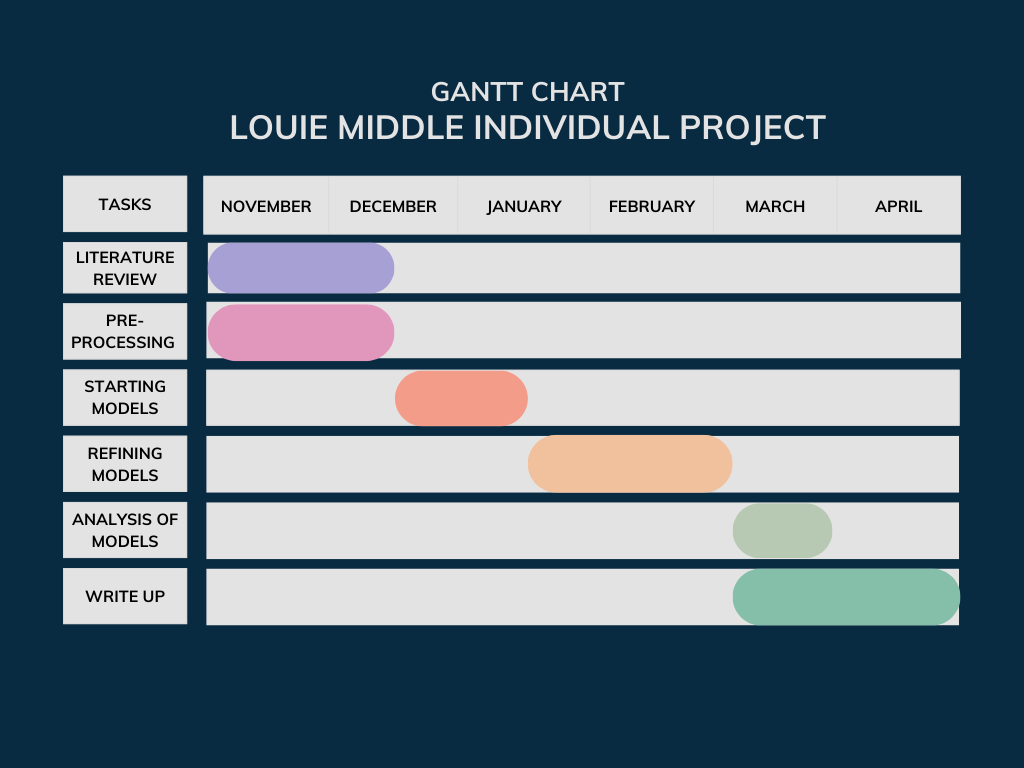
\includegraphics[width=\linewidth]{Gantt Chart.png}
    \caption{Gantt Chart For Project}
    \label{fig:gantt_chart}
\end{figure}

\section{Resources Required}

In order to train any machine learning model an appropriate amount of data for training and testing. 
Because it is not beneficial to use data that is too old \citep{horvat2020}, a recent season's worth of data would be good, saving some data for testing. 

Training machine learning models may also require appropriate computing power depending on the models used and size of the data set. 
This could potentially be achieved with the University of Bath's Hex cluster.

\section[Short Section Title]{Another Section With a Long Title and Whose Title Is Abbreviated in the Table of Contents}

%-------------------------------------------------------------------------------
\begin{table}[htb]
\caption{An example table}
\bigskip
\begin{center}
\label{Example-Table}
\begin{tabular}{|l|l|}
\hline
Items & Values \\
\hline
\hline
Item 1 & Value 1 \\
Item 2 & Value 2 \\
\hline
\end{tabular}
\end{center}
\end{table}

Another section, just for good measure. You can reference a table, figure or equation using \verb|\ref|, just like this reference to Table \ref{Example-Table}.

%%%%%%%%%%%%%%%%%%%%%%%%%%%%%%%%%%%%%%%%%%%%%%%%%%%%%%%%%%%%%%%%%%%%%%%%%%%%%%%%
\section{Example Lists}

%-------------------------------------------------------------------------------
\subsection{Enumerated}

\begin{enumerate}
\item Example enumerated list:
  \begin{itemize}
  \item a nested enumerated list item;
  \item and another one.
  \end{itemize}
\item Second item in the list.
\end{enumerate}

%-------------------------------------------------------------------------------
\subsection{Itemised}

\begin{itemize}
\item Example itemised list.
  \begin{itemize}
  \item A nested itemised list item.
  \end{itemize}
\item Second item in the list.
\end{itemize}

%-------------------------------------------------------------------------------
\subsection{Description}

\begin{description}
\item[Item 1]First item in the list.
\item[Item 2]Second item in the list.
\end{description}


%%%%%%%%%%%%%%%%%%%%%%%%%%%%%%%%%%%%%%%%%%%%%%%%%%%%%%%%%%%%%%%%%%%%%%%%%%%%%%%%
%%%%%%%%%%%%%%%%%%%%%%%%%%%%%%%%%%%%%%%%%%%%%%%%%%%%%%%%%%%%%%%%%%%%%%%%%%%%%%%%
\chapter{Literature and Technology Survey}

\section{Existing Machine Learning in Sport}

\citet{horvat2020} literature review of machine learning in sport for score prediction showed that including too many seasons worth of data for training models reduces the quality of results. 
To those with a basic knowledge of cricket and sport this is not surprising given that in just a few years, many things related to team composition and tactics can change. 
The best prediction results were achieved by researchers who used data from a single season and a data segmentation evaluation method. 
When using data from a single season, most of the data is used for training and a small portion for testing. 
Some researchers used the same data set for training and testing yielding unrealistically accurate results.

The Singlearity-PA model \citep{silver2021baseball} was able to accurately predict the results of a batter versus pitcher plate appearance using a neural-network based AI model. 
The details of the model used are vague, however the network was able to take in 87 inputs and then output probabilities for each of the 21 possible outcomes of a plate appearance (PA) in baseball. 
Comparisons can be made between this and cricket. 
A plate appearance can be compared to an over, comprising 6 balls (or more including no balls and wides) between a single bowler and 1 or more batsmen. 
The outcome of the over could be considered to be the runs scored. 

\citet{silver2021baseball} also split their player base up by how many PAs they had for each player. 
The best players had greater than 500 PAs worth of data each, but the vast majority had less than 100. 
SinglearityPA was able to accurately predict the result of match-ups for these players with fewer PAs better than existing solutions. 
Parallels can be drawn between this and cricket, as there are often players who have little data, yet team selectors would want to know who the best player is to match-up against them.

Extending Singlearity-PA with Markov chains improved more complicated strategies, such as optimal player lineups or to decide on pinch hitters and relief pitchers. 
Similarly, in cricket the batting lineup and choice of bowler at different points in a game have a large impact on the score. 
In the example provided, Singlearity-PA's predicted runs scored for an optimal lineup was 6.7\% better than the actual lineup in the 2019 National League All-Star game. 
It is important not to compare baseball and cricket too closely, but the techniques used by Silver and Huffman could potentially work well in Cricket.

\subsection{Gradient Boosting Methods}

 TODO: Talk about XGBoost in sport

\section{Existing Machine Learning in Cricket}

\citet{KampakisStylianos2015} used Naïve Bayes, logistic regression, random forests and gradient boosted decision trees to predict the outcome of English County 20 over Cricket Matches from 2009 - 2014. 
The performance of each algorithm was assessed using one year's data as the training data set and the following year's data for testing. 
Each model was tested over these seasons and achieved an accuracy of 62.4\% for Naïve Bayes, 60.1\% for logistic regression, 55.6\% for random forests and 57.2\% for decision trees.

\subsection{Existing Machine Learning in the Indian Premier League}

\citet{Saikia2012} have used Artificial Neural Network models to predict the performance of bowlers based on their performance in the first three seasons of the IPL. 
When the predicted results were validated with the players performances in the fourth season, the model had an accuracy of 71.43\%.

\section{Drawbacks of Existing Methods}

Sport outcome predictors are most commonly used by supervised ML methods, typically classification methods or regression methods \citep{horvat2020}. 
Whilst existing research can achieve impressive results, surprises in sport still happen. For example, the odds of Leicester City winning the Premier League in the 2015/2016 season were 1-5000. 
However, analysis of their performances show their title was absolutely deserved.

This could be explained in that a problem with existing models is that they only output a single value. 
There is no uncertainty in the output as to how confident the model is in its prediction. 
This has a problem in that making decisions based on this prediction becomes much more difficult, as decision makers can't be sure how much to trust the prediction. 
Furthermore, certain inputs exist where very little similar training data might exist. 
In such cases, the uncertainty in a models output should be much greater. 
Yet, existing models will still provide a prediction the same as it would for inputs where there was a large amount of training data.

\section{Gaussian Processes in Sport}

TODO: Talk about Gaussian processes in sport

\section{Data Association with Gaussian Processes}

\citep{Kaiser2018}
\citep{Lui2020}
\citep{Blumberg2020}

\subsection{Summary}

A GP is a probabilistic model used for regression and classification tasks in machine learning. 
It models the relationship between inputs and outputs as a random process and makes predictions by modeling the distribution of outputs given the inputs.

First, two kernel objects "pred\_kernel" and "assign\_kernel" are created using the "KERNEL.kern" function. 
These kernels define the covariance function used in the GP model. 
The input dimension, lengthscales, variance, and ARD (Automatic Relevance Determination) flag are set using the "input\_dim", "lengthscales", "variance", and "ARD" arguments, respectively.

The centroids "Z" and "Z\_assign" of the input data "Xtrain" are computed using the k-means clustering algorithm "kmeans", where "num\_ind" is the number of inducing points.

Two GP layers "pred\_layer" and "assign\_layer" are created using the "SVGP\_Layer" class. 
The "pred\_layer" uses the "pred\_kernel" and the "Z" centroids, while the "assign\_layer" uses the "assign\_kernel" and the "Z\_assign" centroids. 
The number of inducing points and outputs is set using the "num\_inducing" and "num\_outputs" arguments.

A Gaussian likelihood object "lik" is created using the "Gaussian" class. 
This likelihood object defines the probability distribution over the outputs.

Finally, a sparse Multi-output Gaussian Process (SMGP) model is created using the "SMGP" class.
The "likelihood" argument is set to "lik", and the "pred\_layer" and "assign\_layer" arguments are set to "pred\_layer" and "assign\_layer" respectively. 
The number of output dimensions "K", the number of Monte Carlo samples "num\_samples", and the number of data points "num\_data" are also specified.

\subsection{Covariance Function}

The covariance function, also known as the kernel function, is a key component in Gaussian Process (GP) models. 
It defines the covariance or similarity between the input points. 
The covariance function models the assumptions about the underlying function that generates the data.

The covariance function takes two inputs, x and x', and returns the covariance between the two inputs. 
This can be interpreted as the degree of similarity between the two inputs. 
The choice of the covariance function determines the type of GP model and its flexibility in fitting the data. 
Common choices for covariance functions include radial basis functions, polynomial functions, and the squared exponential function.

The covariance function can be parameterized by several hyperparameters, such as the lengthscales, which determine the smoothness of the function, and the variance, which determines the magnitude of the output. 
These hyperparameters can be learned during the training process.

In summary, the covariance function in a GP model determines the similarity between the inputs, and is a critical component in defining the assumptions about the underlying function and its flexibility in fitting the data.

\subsection{GP Layers}

TODO: This section can potentially never be mentioned, as now using GPFlow SVGP which isn't called `layer`.

In Gaussian Process (GP) models, layers can be used to define the structure of the model and simplify the modeling process. 
A layer in a GP model typically consists of a set of inducing points, which are used to make predictions about the output. 
The choice of inducing points and the number of inducing points can greatly affect the accuracy and computational efficiency of the GP model.

Layers can be used to model different aspects of the data, such as the mean function and the covariance function. 
The mean function can be modeled as a linear combination of the inputs, while the covariance function can be defined by a radial basis function or a polynomial function.

Layers can also be used to define hierarchical GP models, where different levels of the hierarchy are modeled by different layers. 
This allows the model to capture complex dependencies between the inputs and outputs.

In summary, layers in GP models provide a flexible and powerful way to define the structure of the model and make predictions about the output. 
They can be used to model different aspects of the data, and can help simplify the modeling process while improving the accuracy and computational efficiency of the model.

\subsection{Inducing Points}

In the code you provided, the inducing points are calculated using the k-means clustering method. 
This is because k-means clustering is a commonly used method for selecting a fixed set of representative points that summarize the structure of the data.

The purpose of the inducing points in a Gaussian Process (GP) model is to provide a compact representation of the model that can be used to make predictions about the output. 
The inducing points are typically chosen to be a small subset of the inputs, and the model is defined in terms of the inducing points rather than the inputs themselves. 
This results in a more computationally efficient model that can be trained and used to make predictions faster.

By using the k-means clustering method to calculate the inducing points, the model can take advantage of the structure of the data. 
The k-means algorithm clusters the data into a set of k clusters, where each cluster is represented by its centroid. 
These centroids can be used as the inducing points in the GP model.

In summary, the use of k-means clustering to calculate the inducing points in a GP model is an efficient way to summarize the structure of the data and reduce the dimensionality of the model, while still maintaining its ability to make accurate predictions about the output.

\subsection{Gaussian Likelihood}

TODO: Will need to add a Bernoulli / Multinomial likelihood section?

In a Gaussian Process (GP) model, the likelihood of the data is the probability of observing the data given the model parameters. 
The Gaussian likelihood is a commonly used likelihood function for GP models, and it assumes that the output data is normally distributed.

The Gaussian likelihood is calculated as follows:

Define the mean function, $\mu(x)$, and the covariance function, $K(x, x')$, for the GP model. 
These functions define the structure of the model and determine how the inputs x and outputs y are related.

Calculate the predicted mean, $\mu$, and the predicted covariance, $\Sigma$, of the output data given the inputs and the model parameters. 
This can be done using the mean function and the covariance function.

Calculate the likelihood of the data, $p(y|x, \mu, \Sigma)$, using the predicted mean and covariance. 
The likelihood is given by:

\begin{equation}
    \centering
    p(y|x, \mu, \Sigma) = (2\pi)^(-n/2) * det(\Sigma)^(-1/2) * exp(-1/2 * (y - \mu)^T * \Sigma^(-1) * (y - \mu))
\end{equation}

where $n$ is the number of data points, $y$ is the vector of observed outputs, and $det(\Sigma)$ and $\Sigma^(-1)$ are the determinant and inverse of the covariance matrix $\Sigma$.

The Gaussian likelihood for the entire data-set is then given by the product of the likelihoods of individual data points:

\begin{equation}
    \centering
    p(y|x) = \Pi_i p(y_i|x_i, \mu, \Sigma) 
\end{equation}

In summary, the Gaussian likelihood is calculated by defining the mean function and the covariance function for the GP model, calculating the predicted mean and covariance of the output data, and evaluating the likelihood of the data given the predicted mean and covariance. 
The Gaussian likelihood provides a way to assess the fit of the model to the data, and it is used to determine the optimal values of the model parameters that maximize the likelihood.

\subsection{Prediction and Assignment Layers}

The pred and assign layers in the code you posted are used in a Sparse Variational Gaussian Process (SVGP) model. 
SVGP is a type of GP model that is used to handle large datasets, where computing the covariance matrix of all data points is computationally infeasible.

The main idea behind SVGP is to use a smaller number of inducing points to represent the covariance structure of the entire dataset. 
The pred and assign layers in the code represent two separate models for predicting the outputs of the GP.

The pred layer is used for prediction, i.e., to make predictions for new inputs. 
This layer models the covariance between the inducing points and the input points. 
The inducing points are obtained using a clustering method, such as k-means, and they are used to represent the entire dataset.

The assign layer is used to assign each data point to the closest inducing point, based on the similarity between the data points and the inducing points. 
This layer models the covariance between the data points and the inducing points, and it allows the GP to capture the relationship between the data points and the inducing points.

In summary, the pred and assign layers are used to make predictions and assign data points to the closest inducing points in a SVGP model, respectively. 
These layers allow the GP to handle large datasets efficiently and effectively.

%% NOTE Replace the following with chapters that are appropriate for your
%%      style of project.  It is unlikely these will fit your project perfectly.

%%%%%%%%%%%%%%%%%%%%%%%%%%%%%%%%%%%%%%%%%%%%%%%%%%%%%%%%%%%%%%%%%%%%%%%%%%%%%%%%
%%%%%%%%%%%%%%%%%%%%%%%%%%%%%%%%%%%%%%%%%%%%%%%%%%%%%%%%%%%%%%%%%%%%%%%%%%%%%%%%
\chapter{Requirements}

If you are doing a primarily software development project, this is the chapter in which you review the requirements decisions and critique the requirements process.

%%%%%%%%%%%%%%%%%%%%%%%%%%%%%%%%%%%%%%%%%%%%%%%%%%%%%%%%%%%%%%%%%%%%%%%%%%%%%%%%
%%%%%%%%%%%%%%%%%%%%%%%%%%%%%%%%%%%%%%%%%%%%%%%%%%%%%%%%%%%%%%%%%%%%%%%%%%%%%%%%
\chapter{Design}

This is the chapter in which you review your design decisions at various
levels and critique the design process.

%%%%%%%%%%%%%%%%%%%%%%%%%%%%%%%%%%%%%%%%%%%%%%%%%%%%%%%%%%%%%%%%%%%%%%%%%%%%%%%%
%%%%%%%%%%%%%%%%%%%%%%%%%%%%%%%%%%%%%%%%%%%%%%%%%%%%%%%%%%%%%%%%%%%%%%%%%%%%%%%%
\chapter{Implementation and Testing}

This is the chapter in which you review the implementation and testing decisions and issues, and critique these processes.

Code can be output inline using \verb@\lstinline|some code|@.  For example, this code is inline: \lstinline|public static int example = 0;| (we have used the character \verb@|@ as a delimiter, but any non-reserved character not in the code text can be used.)

Code snippets can be output using the \verb|\begin{lstlisting} ... \end{lstlisting}|
environment with the code given in the environment. For example, consider listing \ref{Example-Code}, below.

\begin{lstlisting}[breaklines,breakatwhitespace,caption={Example code},label=Example-Code]
public static void main() {

  System.out.println("Hello World");

}
\end{lstlisting}

Code listings are produced using the package `listings'.  This has many useful options, so have a look at the package documentation for further ideas.

%%%%%%%%%%%%%%%%%%%%%%%%%%%%%%%%%%%%%%%%%%%%%%%%%%%%%%%%%%%%%%%%%%%%%%%%%%%%%%%%
%%%%%%%%%%%%%%%%%%%%%%%%%%%%%%%%%%%%%%%%%%%%%%%%%%%%%%%%%%%%%%%%%%%%%%%%%%%%%%%%
\chapter{Results}

This is the chapter in which you review the outcomes, and critique the outcomes process. You may include user evaluation here too.

%%%%%%%%%%%%%%%%%%%%%%%%%%%%%%%%%%%%%%%%%%%%%%%%%%%%%%%%%%%%%%%%%%%%%%%%%%%%%%%%
%%%%%%%%%%%%%%%%%%%%%%%%%%%%%%%%%%%%%%%%%%%%%%%%%%%%%%%%%%%%%%%%%%%%%%%%%%%%%%%%
\chapter{Conclusions}

%%
%% Now we are back to the standard project contents that you should include
%%

This is the chapter in which you review the major achievements in the light of your original objectives, critique the process, critique your own learning and identify possible future work.

%%%%%%%%%%%%%%%%%%%%%%%%%%%%%%%%%%%%%%%%%%%%%%%%%%%%%%%%%%%%%%%%%%%%%%%%%%%%%%%%
%%%%%%%%%%%%%%%%%%%%%%%%%%%%%%%%%%%%%%%%%%%%%%%%%%%%%%%%%%%%%%%%%%%%%%%%%%%%%%%%
\bibliography{BibFile}

%%%%%%%%%%%%%%%%%%%%%%%%%%%%%%%%%%%%%%%%%%%%%%%%%%%%%%%%%%%%%%%%%%%%%%%%%%%%%%%%
%%%%%%%%%%%%%%%%%%%%%%%%%%%%%%%%%%%%%%%%%%%%%%%%%%%%%%%%%%%%%%%%%%%%%%%%%%%%%%%%
\appendix

%%
%% Use the appendix for major chunks of detailed work, such as these. Tailor
%% these to your own requirements
%%

%%%%%%%%%%%%%%%%%%%%%%%%%%%%%%%%%%%%%%%%%%%%%%%%%%%%%%%%%%%%%%%%%%%%%%%%%%%%%%%%
%%%%%%%%%%%%%%%%%%%%%%%%%%%%%%%%%%%%%%%%%%%%%%%%%%%%%%%%%%%%%%%%%%%%%%%%%%%%%%%%
\chapter{Design Diagrams}

%%%%%%%%%%%%%%%%%%%%%%%%%%%%%%%%%%%%%%%%%%%%%%%%%%%%%%%%%%%%%%%%%%%%%%%%%%%%%%%%
%%%%%%%%%%%%%%%%%%%%%%%%%%%%%%%%%%%%%%%%%%%%%%%%%%%%%%%%%%%%%%%%%%%%%%%%%%%%%%%%
\chapter{User Documentation}

%%%%%%%%%%%%%%%%%%%%%%%%%%%%%%%%%%%%%%%%%%%%%%%%%%%%%%%%%%%%%%%%%%%%%%%%%%%%%%%%
%%%%%%%%%%%%%%%%%%%%%%%%%%%%%%%%%%%%%%%%%%%%%%%%%%%%%%%%%%%%%%%%%%%%%%%%%%%%%%%%
\chapter{Raw Results Output}

%%%%%%%%%%%%%%%%%%%%%%%%%%%%%%%%%%%%%%%%%%%%%%%%%%%%%%%%%%%%%%%%%%%%%%%%%%%%%%%%
%%%%%%%%%%%%%%%%%%%%%%%%%%%%%%%%%%%%%%%%%%%%%%%%%%%%%%%%%%%%%%%%%%%%%%%%%%%%%%%%
\chapter{Code}

%% NOTE For this to typeset correctly, ensure you use the pdflatex
%%      command in preference to the latex command.  If you do not have
%%      the pdflatex command, you will need to remove the landscape and
%%      multicols tags and just make do with single column listing output

\begin{landscape}
\begin{multicols}{2}
\section{File: yourCodeFile.java}
\lstinputlisting[basicstyle=\scriptsize]{yourCodeFile.java}
\end{multicols}
\end{landscape}

\end{document}
